%%%%%%%%%%%%%%%%%%%%%%%%%%%%%%%%

\documentclass[11pt,a4paper]{article}
\usepackage{times}
\usepackage[utf8]{inputenc}
\usepackage[croatian]{babel}
\usepackage[T1]{fontenc} % Latin Modern

%%%%%%%%%%%%%%%%%%%%%%%%%%%%%%%%


%%%%%%%%%%%%%%%%%%%%%%%%%%%%%%%%
%%%%%%%%  MATEMATICKI PAKETI %%%%%%%%%%%
%%%%%%%%%%%%%%%%%%%%%%%%%%%%%%%%

\usepackage{amsmath}
\usepackage{amsfonts}
\usepackage{amssymb}
\usepackage{esvect}

%%%%%%%%%%%%%%%%%%%%%%%%%%%%%%%%

%%%%%%%%%%%%%%%%%%%%%%%%%%%%%%%%
%%%%%%%%%% PAKETI ZA SLIKE  %%%%%%%%%%%%
%%%%%%%%%%%%%%%%%%%%%%%%%%%%%%%%

\usepackage{graphicx}
\usepackage{float}
\usepackage[hidelinks]{hyperref}
\usepackage{caption}
\usepackage{subcaption}
\usepackage{booktabs}


%%%%%%%%%%%%%%%%%%%%%%%%%%%%%%%%

%%%%%%%%%%%%%%%%%%%%%%%%%%%%%%%%
%%%%%%%%%    PRORED 1.5   %%%%%%%%%%%%%%
%%%%%%%%%%%%%%%%%%%%%%%%%%%%%%%%

\renewcommand{\baselinestretch}{1.5}

%%%%%%%%%%%%%%%%%%%%%%%%%%%%%%%%


%%%%%%%%%%%%%%%%%%%%%%%%%%%%%%%%
%%%%%%%%%% TABLICA - ANTUN %%%%%%%%%%%%
%%%%%%%%%%%%%%%%%%%%%%%%%%%%%%%%

\usepackage{array}
\usepackage{multirow}
\newcolumntype{C}[1]{>{\centering\let\newline\\\arraybackslash\hspace{0pt}}m{#1}}
\newcolumntype{L}[1]{>{\raggedright\let\newline\\\arraybackslash\hspace{0pt}}m{#1}}
\newcolumntype{R}[1]{>{\raggedleft\let\newline\\\arraybackslash\hspace{0pt}}m{#1}}
\usepackage{ctable}

%%%%%%%%%%%%%%%%%%%%%%%%%%%%%%%%

%%%%%%%%%%%%%%%%%%%%%%%%%%%%%%%%
%%%%%%%%%% TABLICA - MARTINA %%%%%%%%%%%
%%%%%%%%%%%%%%%%%%%%%%%%%%%%%%%%

\makeatletter
\renewcommand*\env@matrix[1][\arraystretch]{%
  \edef\arraystretch{#1}%
  \hskip -\arraycolsep
  \let\@ifnextchar\new@ifnextchar
  \array{*\c@MaxMatrixCols c}}
\makeatother



%%%% LATEX KOD ZA KORISTENJE TABLICE %%%%
%%% PRIMJER %%%

%\setlength\extrarowheight{1pt}
%\begin{table}[h]
%\centering
%\caption{Tablica s prikazom }
%\label{prva}
%\begin{tabular}{|l|c|}
%\hline
%\textbf{txt} &  \\ \hline 
%txt & txt    \\ 
%txt & txt   \\ \hline
%txt & txt    \\ \hline
%\end{tabular}
%\end{table}

%%%%%%%%%%%%%%%%%%%%%%%%%%%%%%%%


%%%%%%%%%%%%%%%%%%%%%%%%%%%%%%%%
%%%%%%% DIO ZA UNOS ISJECAKA KODA %%%%%%%%
%%%%%%%%%%%%%%%%%%%%%%%%%%%%%%%%

\usepackage{listings}
\usepackage{color}
 
\definecolor{codegreen}{rgb}{0,0.6,0}
\definecolor{codegray}{rgb}{0.5,0.5,0.5}
\definecolor{codepurple}{rgb}{0.58,0,0.82}
 
\lstdefinestyle{mystyle}{   
    commentstyle=\color{codegreen},
    keywordstyle=\color{blue},
    numberstyle=\tiny\color{codegray},
    stringstyle=\color{codepurple},
    basicstyle=\footnotesize,
    breakatwhitespace=false,         
    breaklines=true,                 
    captionpos=b,                    
    keepspaces=true,                 
    numbers=left,                    
    numbersep=5pt,                  
    showspaces=false,                
    showstringspaces=false,
    showtabs=false,                  
    tabsize=1
}
 
\lstset{style=mystyle}

%\lstinputlisting[language=Matlab, firstline=1, lastline=4, numbers=left, frame=single, label={lst:prvi}, caption={Diskretizacija sustava korištenjem Matlaba}, captionpos=b]{peti.m} 

%%%%%%%%%%%%%%%%%%%%%%%%%%%%%%%%


%----------------------------
% za uredjenje stranice
\usepackage[left=2.5cm,right=2.5cm,top=2.5cm,bottom=2.5cm]{geometry}
\usepackage{fancyhdr}
\pagestyle{fancy} 
\lhead{\leftmark}
\rhead{\rightmark}
\usepackage{titlesec} %za točku iza broja sectiona
\titleformat{\section}{\huge\bfseries}{\thetitle.\quad}{0em}{}
\titleformat{\subsection}{\LARGE\bfseries}{\thetitle.\quad}{0em}{}
\titleformat{\subsubsection}{\Large\bfseries}{\thetitle.\quad}{0em}{}
\titleformat{\paragraph}
{\normalfont\large\bfseries}{\thetitle.\quad}{1em}{}
\titlespacing*{\paragraph}
{0pt}{3.25ex plus 1ex minus .2ex}{1.5ex plus .2ex}
\setcounter{secnumdepth}{5}

\usepackage{indentfirst} %uvlacenje prvog paragrafa
% primjer pozivanja sectiona
% \section*{UVOD} \pdfbookmark{UVOD}{section:UVOD}

\usepackage{tocloft}
\usepackage{import}
\usepackage{standalone}
\graphicspath{{Uvod/}, {Ciljevi/}, {Materijal/}, {Rasprava/}, {Rezultati/}} 

\hypersetup{
  colorlinks   = true, %Colours links instead of ugly boxes
  urlcolor     = black, %Colour for external hyperlinks
  linkcolor    = black, %Colour of internal links
  citecolor   = blue %Colour of citations
}

\usepackage{subcaption}
\usepackage{lscape}
\begin{document}

U ovom poglavlju opisana je mehanička konstrukcija letjelice. Osnova je postojeća laboratorijska letjelica  \textit{ArduCopter}. Letjelica  \textit{ArduCopter} standarnog je dizajna, s četiri pogonska \textit{beskolektorska DC} motora s pripadnim  elektroničkim upravljačima brzine(\textit{ESC - eng. Electronic Speed Control}). Zbog jednostavnog i modularnog dizajna, letjelica je prikladna platforma za razne promjene i proširenja raznim upravljačkim uređajima, senzorima i aktuatorima. U \textit{LARICS} laboratoriju trenutno postoji nekoliko modela letjelica ovog tipa koje se koriste za većinu eksperimenata. Dizajn i veličina letjelice prikladna je za većinu eksperimenata koji se provode u laboratoriju, uključujući planiranje i izvođenje trajektorija u prostoru, manipulaciju objekata i drugo. Upravo zato odlučeno je modificirati jednu od postojećih konstrukcija te izraditi platformu za eksperimentalno testiranje novog koncepta upravljanja višerotorskom letjelicom. Glavna modifikacija odnosi se na dizajniranje i izradu mehanizma kojim će se omogućiti pomak mase na kraku. Također, potrebno je smjestiti sve ostale komponente nužne za upravljanje letjelicom, poput kontrolera leta i upravljačkog sklopovlja pomičnih masa. Za izradu dizajna korišten je CAD alat. Konačni 3D izgled modificirane letjelice prikazan je Slikom \ref{Slika:3D_drone_final}.

\begin{figure}[H]
	\centering
	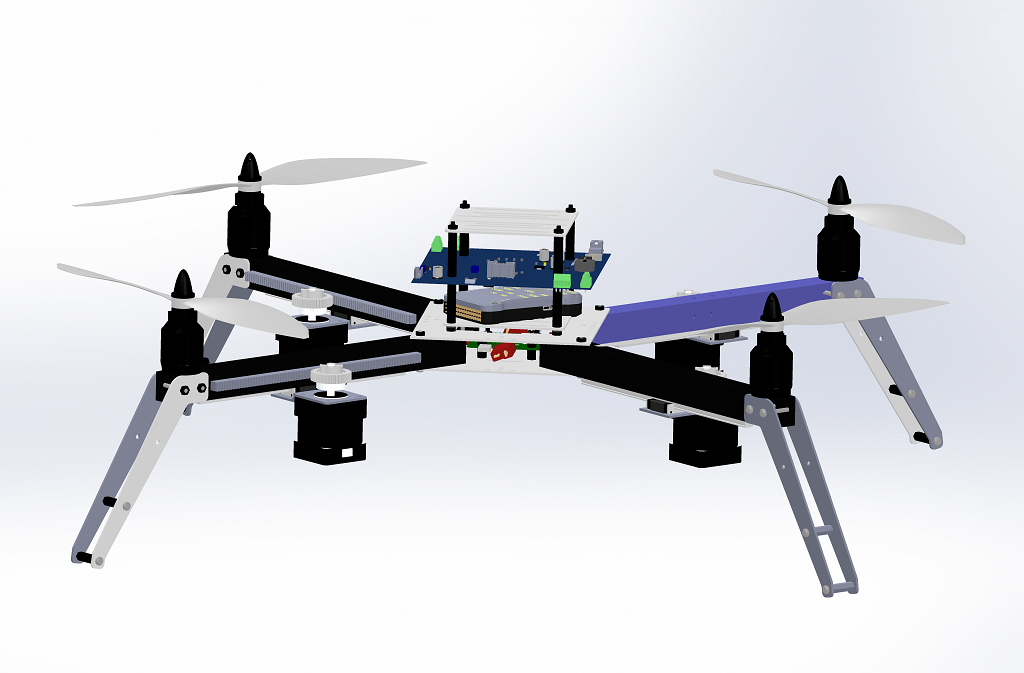
\includegraphics[width=0.9\textwidth]{figures/arducopter_with_PCB.png}
	\caption{3D model modificirane letjelice \textit{ArduCopter}}
	\label{Slika:3D_drone_final}
\end{figure}

\subsection{Letjelica  \textit{ArduCopter}}

Osnova konstrukcije letjelice s pomičnim masama je multirotorska letjelica  \textit{ArduCopter}, prikazano Slikom \ref{fig:3D_drone_original}.  \textit{ArduCopter} je laboratorijska letjelica pogonjena s 4 \textit{beskolektorska DC} motora. Klasičnim konceptom upravljanja, brzom promjenom brzina vrnje motora, ostvaruju se zadani kutevi i kutne brzine letjelice. Letjelica ima modularan dizajn, što omogućava jednostavne nadogradnje, poput različitih upravljačkih uređaja, senzora i aktuatora. Sva proširenja letjelice dodaju se jedno iznad drugoga na već predviđene položaje iznad razine krakova u centru letjelice. Zbog svega navedenog,  \textit{ArduCopter} je odabran kao osnovna platforma za izradu multirotorske letjelice s pomičnim masama.

\medskip

Postojeća mehanička konstrukcija letjelice  \textit{ArduCopter} se u potpunosti koristi, a obuhvaća: 
\begin{center}
	\begin{itemize}
		\item Tijelo letjelice uključujući razvodnu ploču za napajanje iz baterije i prihvat slojeva za proširenje
		\item 4 aluminijska kraka
		\item 4 plastična zaustavna kraka
		\item 4  \textit{beskolektorska DC} motora s pripadnim \textbf{ESC} pogonima
		\item 4 plastična propelera
	\end{itemize}
\end{center}

\subsubsection*{Modifikacija postojeće letjelice}
Predstavljenu postojeću letjelicu \textit{ARDUCOPTER} potrebno je modificirati na sljedeći način:
\begin{center}
	\begin{itemize}
		\item Dodati 4 pokretne mase, odabrati aktuatore, konstruirati i izraditi mehanizam kretanja mase po kraku letjelice.
		\item Dodati kontroler leta \textit{Pixhawk PX4}, za kompletno upravljanje letjelicom s pokretnim masama
		\item Izraditi elektroničko slopovlje potrebno za pogon masa, realizirati komunikaciju s kontrolerom leta te dodati mogućnosti za daljnja funkcionalna proširenja letjelice.
	\end{itemize}
\end{center}


\begin{figure}[H]
	\centering
	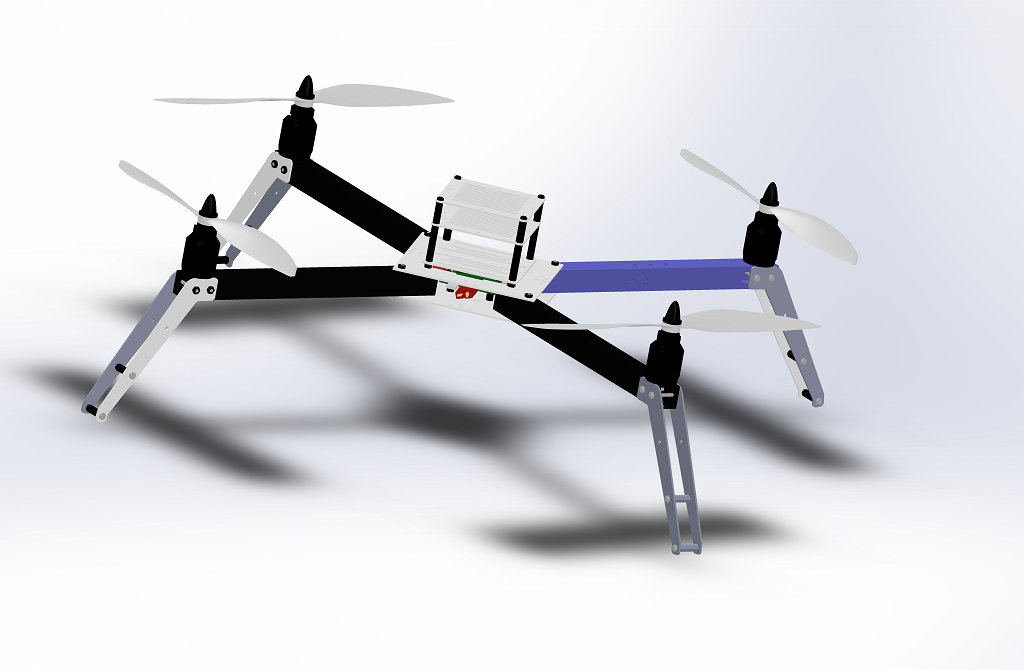
\includegraphics[width=0.9\textwidth]{figures/arducopter_original.png}
	\caption{3D model postojeće letjelice \textit{ArduCopter}}
	\label{fig:3D_drone_original}
\end{figure}

\subsection{Klizni mehanizam pokretne mase}

Budući da se novi koncept upravljanja letjelice zasniva na promjeni centra mase, koje je realizirano pomičnim masama na krakovima, potrebno je izraditi mehanizam kretanja pokretne mase po kraku letjelice. Kretanje pomične mase je linijsko, a mehanizam kretanja mora biti realiziran s minimalnim trenjem. Kretanje pokretne mase ostvareno je električnim aktuatorom.

\subsubsection{Aktuator}
Zadaća je aktuatora pokretne mase gibanje mase po kraku letjelice, čime se ostvaruje promjena centra mase letjelice. Kako bi ukupna masa letjelice bila manja, sam aktuator na svakom kraku se koristi kao pokretna masa. Za aktuator je odabran koračni motor \textit{NEMA 14}, prikazan slikom \ref{fig:stepper_motor}. Specifikacije koračnog motora su prikazane tablicom \ref{tab:specifikacija_steppera}.

\begin{figure}[H]
	\centering
	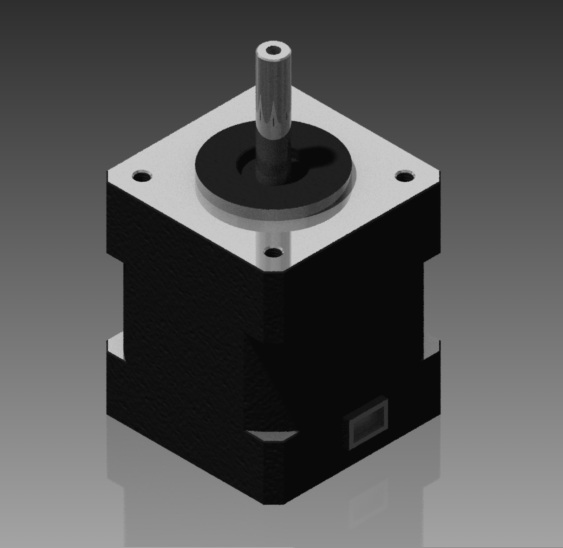
\includegraphics[width=0.3\textwidth]{figures/StepperMotor.jpg}
	\caption{Koračni motor}
	\label{fig:stepper_motor}
\end{figure}


\begin{table}[H]
	\centering
	\caption{Specifikacije koračnog motora }
	\label{tab:specifikacija_steppera}
	\begin{tabular}{|l|c|}
		\hline
		\textbf{Proizvođač} &PROIZVOĐAČ \\ \hline 
		\textbf{Model} & NEMA 14  \\ \hline 
		\textbf{Veličina} & 35mm x 35mm x 36mm, neuključujući osovinu  \\ \hline 
		\textbf{Masa} & 180 g  \\ \hline 
		\textbf{Promjer osovine} & 5 mm \\ \hline 
		\textbf{Broj koraka po okretu} & 200 \\ \hline 
		\textbf{Broj faza} & 2 \\ \hline 
		\textbf{Current rating} & 1A po fazi \\ \hline 
		\textbf{Moment zadržavanja} & 1.4 $kg/cm$ \\ \hline 
		\textbf{Moment inercije rotora} & 14 $g/cm^2$ \\ \hline 
	\end{tabular}
\end{table}

Koračni motor odabran je zato jer pruža mogućnost korištenja upravljanja pozicijom motora u otvorenoj petlji. Točnije, pravilnim upravljanjem i brojanjem koraka koje je motor napravio, moguće je u svakom trenutku znati u kojem položaju se motor nalazi te samim time i na kojoj poziciji se nalazi pokretna masa. Ako bi se koristio neki drugi tip motora, bilo bi potrebno dodati senzore poput enkodera kako bi se moglo pratiti kretanje i položaj mase na kraku.




\subsubsection{Kretanje po kraku letjelice}

Kretanje mase po kraku je linijsko. Kako bi kretanje mase imalo minimalno trenje, odabran je klizni mehanizam prikazan slikom \ref{fig:klizni_mehanizam}. Klizni mehanizam montiran je s doljnje strane kraka, a za aluminijsku kvadratnu cijev pričvršćen je s dva vijka. Klizni mehanizam se sastoji od vodilice i kolica. Na kolicima se nalazi klizni mehanizam koji se sastoji od sitnih kuglica koje omogućavaju klizno gibanje s malim trenjem. Na kolica kliznog mehanizma montirano je posebno konstruiran prihvat koračnog motora(slika \ref{fig:stepper_bracket}), kojim se koračni motor učvršćuje na klizni mehanizam.


\begin{figure}[H]
\centering
\begin{minipage}{.5\textwidth}
  \centering
  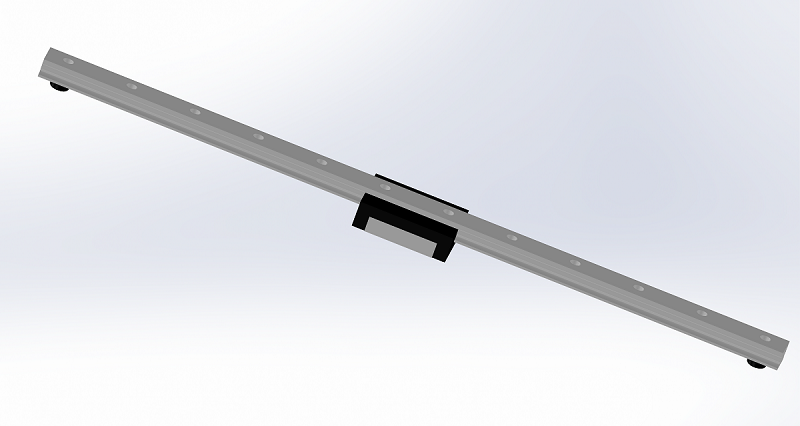
\includegraphics[width=.9\linewidth]{figures/linear_guide_7mm.png}
  \captionof{figure}{Klizni mehanizam}
  \label{fig:klizni_mehanizam}
\end{minipage}%
\begin{minipage}{.5\textwidth}
  \centering
  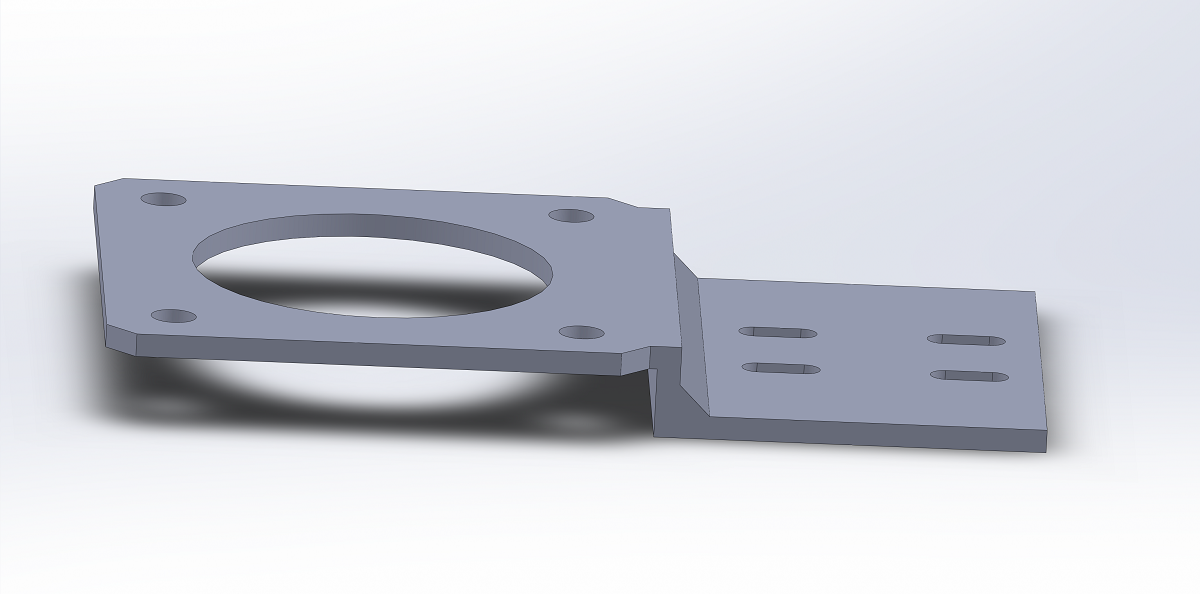
\includegraphics[width=.9\linewidth]{figures/stepper_bracket.png}
  \captionof{figure}{Prihvat koračnog motora}
  \label{fig:stepper_bracket}
\end{minipage}
\end{figure}

Rotacija koračnih motora se prenosi na linijsko gibanje po kraku pomoću zupčastog prijenosa. Zupčasti prijenos je dizajniran tako da jedan puni okret koračnog motora pokriva cijeli potrebni raspon linijskog gibanje na kraku. 
Zupčasta letva(slika \ref{fig:gear_rack}) je zaljepljena na bočnu stranu aluminijske kvadratne cijevi pomoću dvokomponentnog ljepila. Zupčanik(slika \ref{fig:gear_gear}) se montira na adapter osovine koračnog motora pomoću 4 vijka. 



\begin{figure}[H]
\centering
\begin{subfigure}{.5\textwidth}
  \centering
  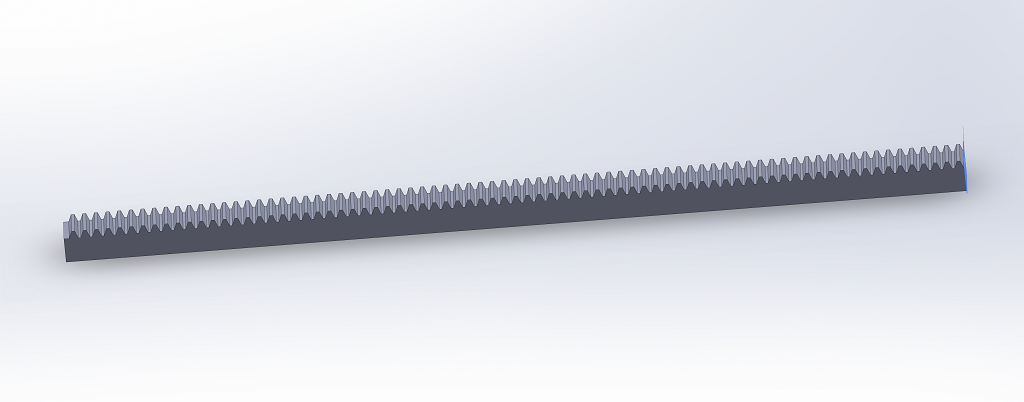
\includegraphics[width=.9\linewidth]{figures/gear_rack_6mm.png}
  \caption{Zupčasta letva}
  \label{fig:gear_rack}
\end{subfigure}%
\begin{subfigure}{.5\textwidth}
  \centering
  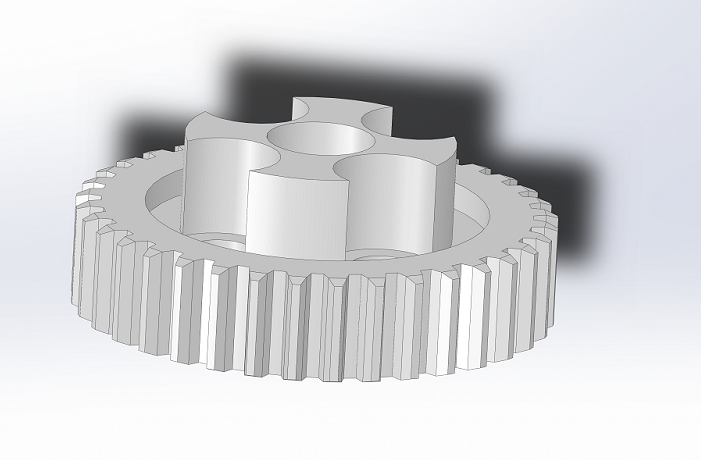
\includegraphics[width=.9\linewidth]{figures/gear_25_07.png}
  \caption{Zupčanik}
  \label{fig:gear_gear}
\end{subfigure}

\caption{Prikaz elemenata zupčastog prijenosa}
\label{fig:gear}
\end{figure}


\subsubsection{Izrada i montaža}

Za dizajniranje mehaničke konstrukcije korišten je CAD alat, koji omogućava 3D modeliranje svih dijelova od kojih je izrađena letjelica. Nakon dizajniranja svakog pojedinog dijela, prelazi se na spajanje dijelova u veće cjeline. Prednost 3D modeliranja je trenutni pregled izgleda konstrukcije, kao i mogućnost izvoza svakog pojedinog dijela u neki od standardnih formata. 

U izradi nekih dijelova konstrukcije korištena je tehnologija 3D printanja. 3D printanje jednostavno je i efikasno rješenje u izradi prototipa. Nakon izrade 3D modela u nekom od CAD alata, radi se priprema pojedinog elementa za izradu. Priprema uključuje učitavanje elementa u poseban softver proizvođača 3D printera. Nakon postavljanja svih parametara izrade poput preciznosti, ispunjenosti i dr. slijedi izvoz podataka u standardan \textit{gcode} format koji koristi 3D printer. Nakon toga slijedi izrada koja je u potpunosti automatizirana.

Dodatno, za montažu kliznih mehanizama na aluminijske kvadratne cijevi potrebno je precizno izbušiti rupe, kroz koje će se pomoću vijka pričvrstiti klizni mehanizam. Zbog toga je korišten CNC stroj.

Nakon pripreme svih dijelova, slijedi montaža. Slikom \ref{fig:arm_assembly} prikazan je konačni 3D model pokretne mase na kraku letjelice.


\begin{figure}[H]
\centering
\begin{subfigure}{.5\textwidth}
  \centering
  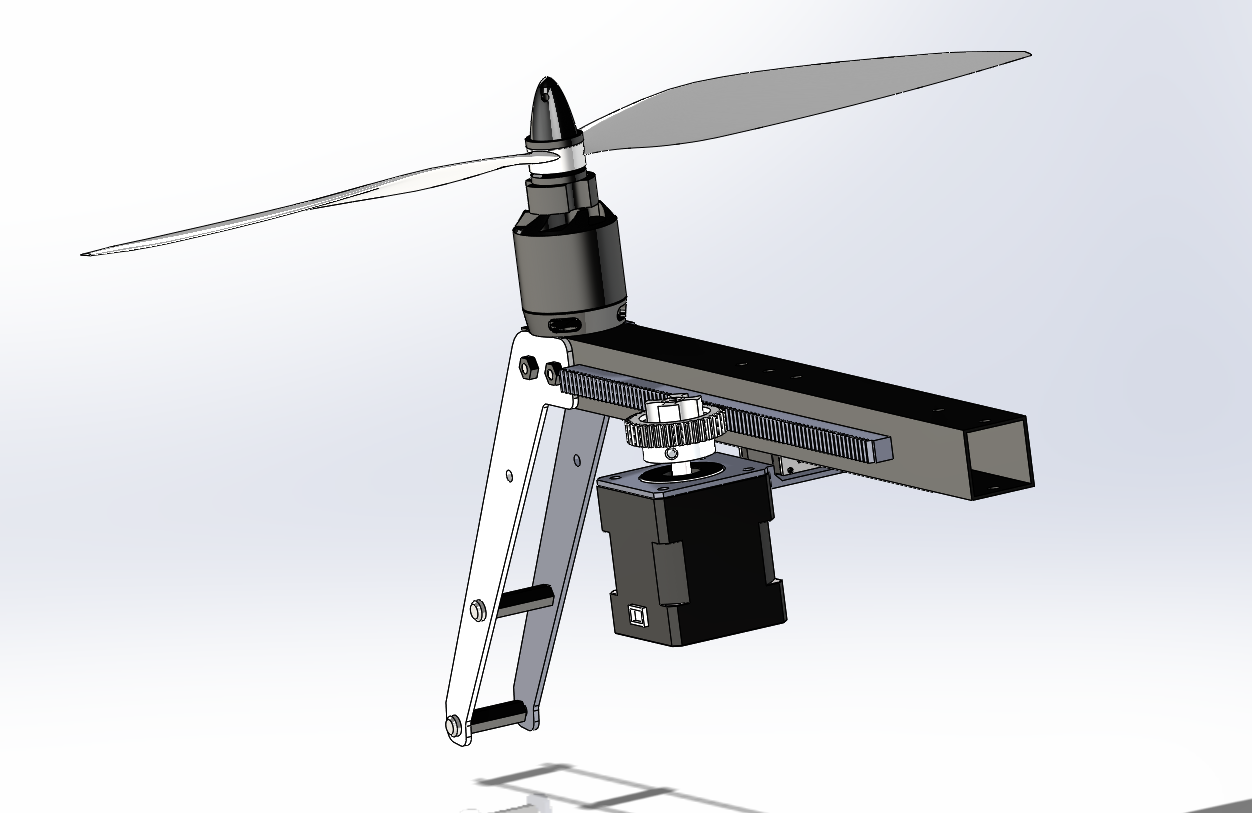
\includegraphics[width=.9\linewidth]{figures/arm_assembly1.png}
  \caption{Pogled 1}
  \label{fig:sub1}
\end{subfigure}%
\begin{subfigure}{.5\textwidth}
  \centering
  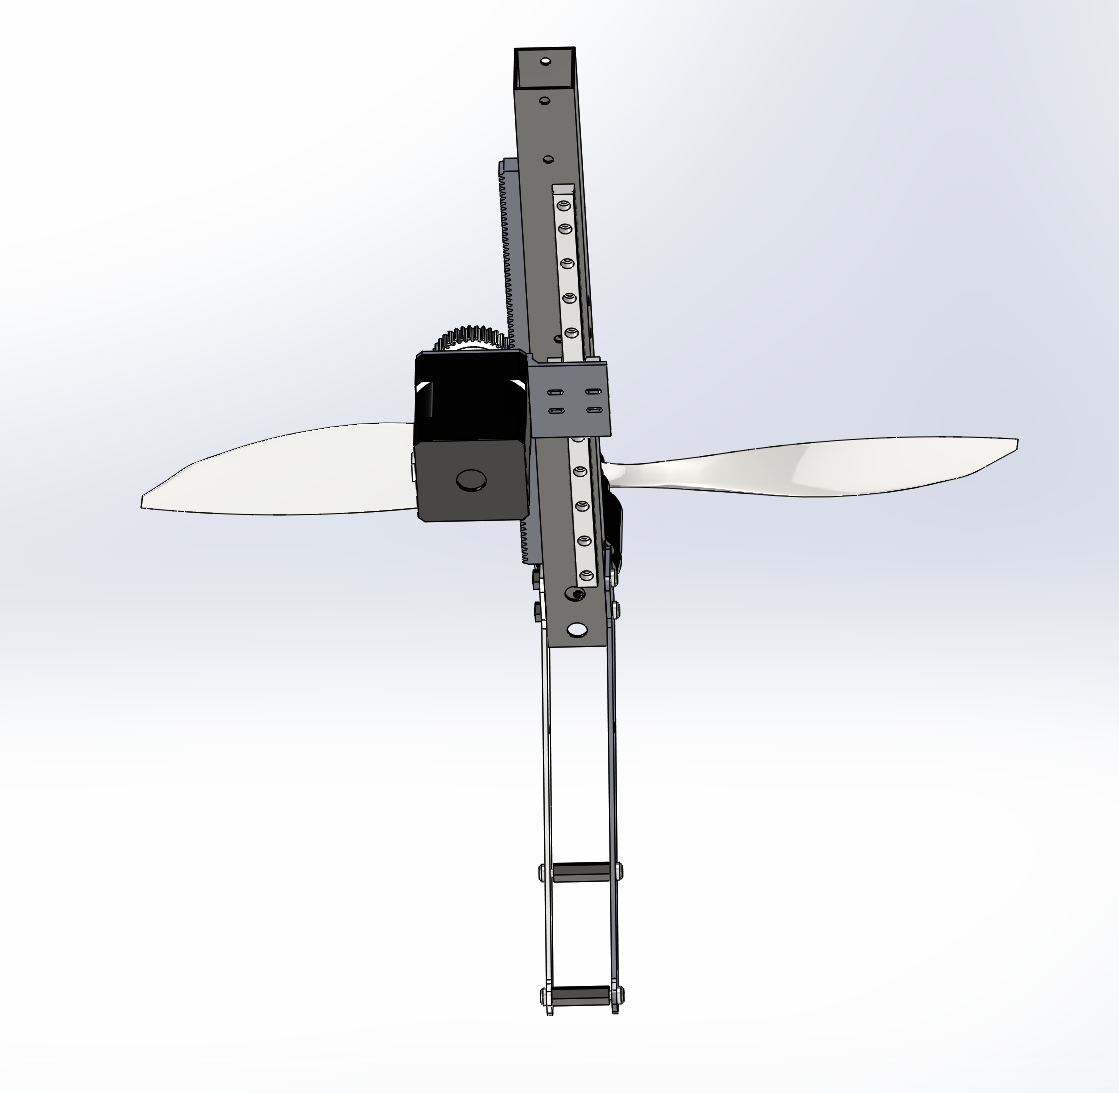
\includegraphics[width=.9\linewidth]{figures/arm_assembly2.png}
  \caption{Pogled 2}
  \label{fig:sub2}
\end{subfigure}
\caption{Prikaz 3D modela jednog kraka letjelice s pomičnom masom}
\label{fig:arm_assembly}
\end{figure}


Nakon montaže svih dijelova, modificirana letjelica \textit{ArduCopter} postavljena je na stalak, s omogućenim jednim stupnjem slobode. Konačni izgled letjelice postavljene na stalak prikazan je Slikom \ref{fig:arm_assembly_Real}.

\begin{figure}[H]
	\centering
	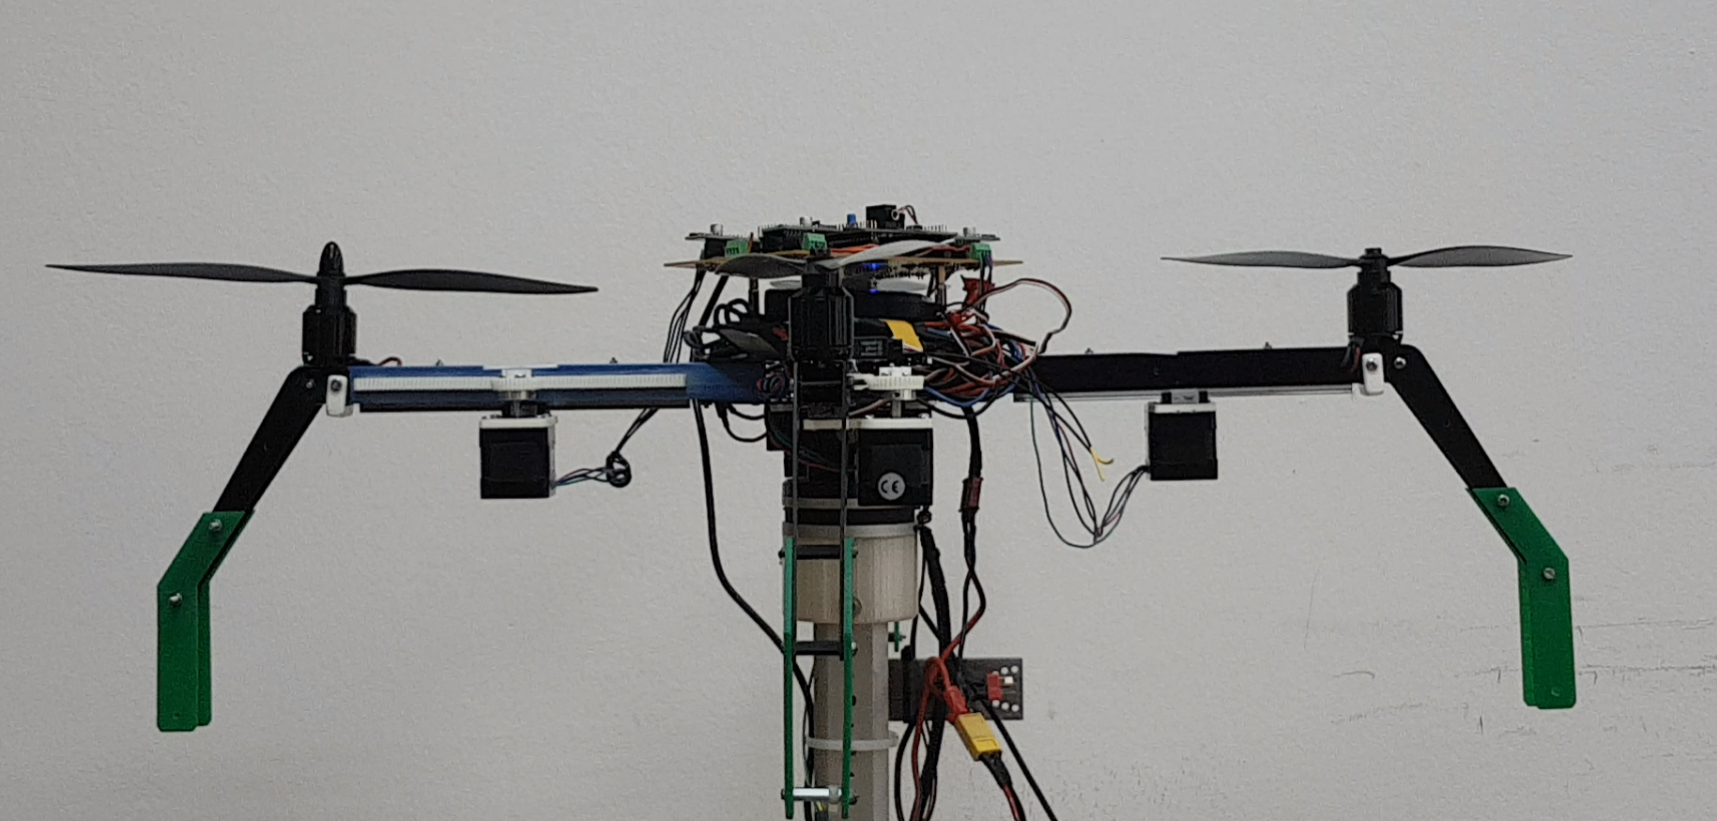
\includegraphics[width=0.9\textwidth]{figures/letjelica.png}
	\caption{Prikaz laboratorijskog modela letjelice s pomičnom masom}
	\label{fig:arm_assembly_Real}
\end{figure}



\subsection{Horizontalna montaža sastavnih dijelova letjelice}
Modularni dizajn letjelice \textit{ArduCopter} omogućava jednostavno proširenje letjelice. Iznad ravnine krakova moguće je dodavati razne slojeve. Slojevi su razmaknuti distancerima s navojem M3. 

\subsubsection{Sloj kontrolera leta}

Kontroler leta \textit{Pixhawk} se koristi za cjelokupno upravljanje letjelicom. U samom kontroleru su ugrađeni svi potrebni senzori za let, poput žiroskopa, akcelerometra i dr. Kontroler leta potrebno je postaviti što bliže osima rotacije letjelice. U ovom slučaju kontroler je postavljen neposredno iznad ravnine krakova. Položaj kontrolera leta prikazan je slikom \ref{fig:slot_pixhawk}.

\begin{figure}[H]
	\centering
	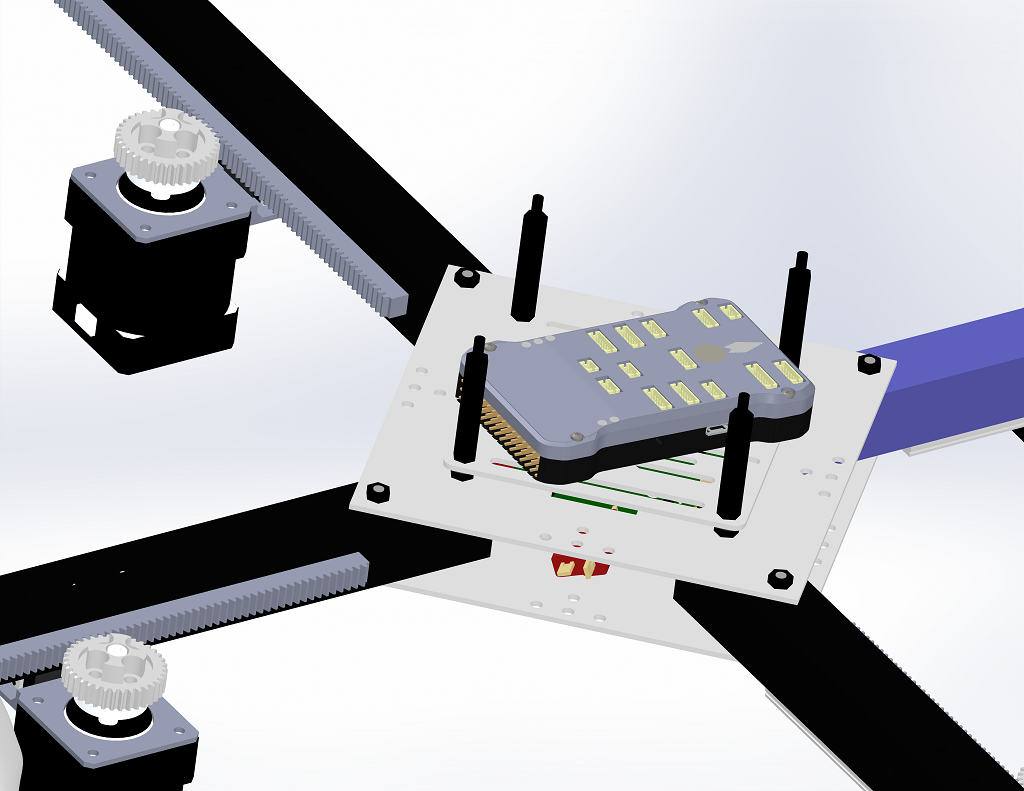
\includegraphics[width=0.7\textwidth]{figures/arducopter_slot_pixhawk.png}
	\caption{Sloj kontrolera leta}
	\label{fig:slot_pixhawk}
\end{figure}


\subsubsection{Sloj upravljačkog sklopovlja}

Iznad kontolera leta postavljeno je posebno izrađeno elektroničko slopovlje za upravljanje koračnim motorima. Dimenzija tiskane pločice jednaka je dimenziji bazne ploče koja se nalazi u ravnini krakova. Pločica je 
razmaknuta od kontrolera leta pomoću distancera. Pozicioniranje upravljačkog sklopovlja prikazano je Slikom \ref{fig:slot_pcb}.


\begin{figure}[H]
	\centering
	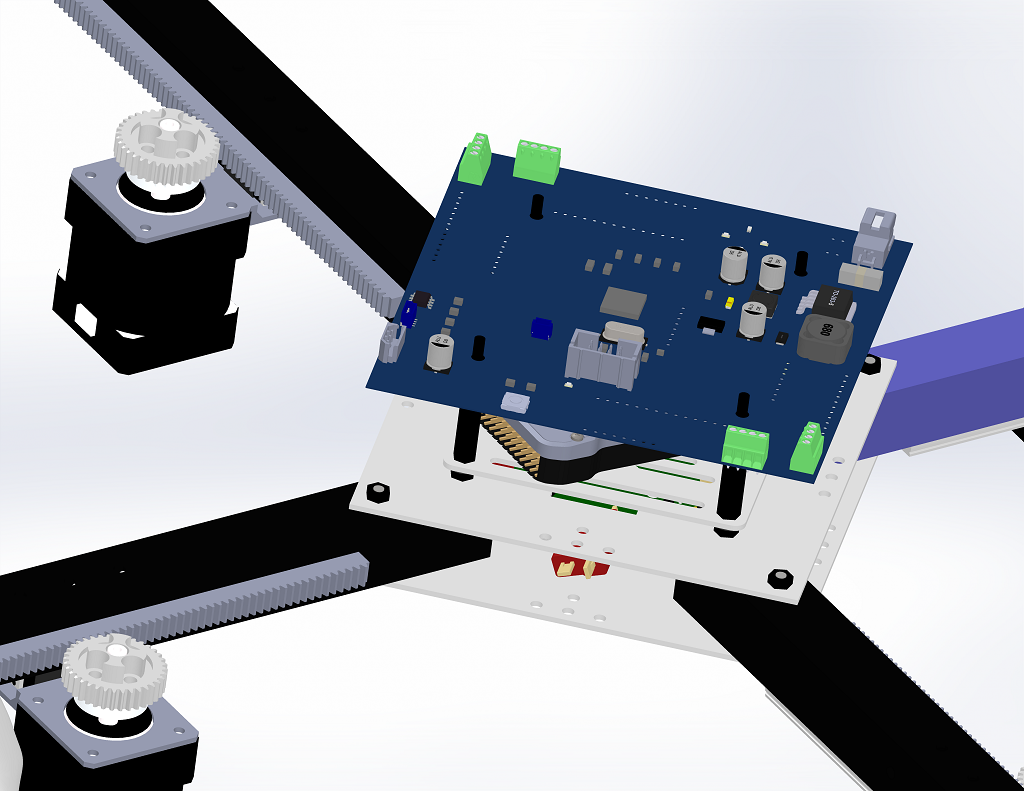
\includegraphics[width=0.7\textwidth]{figures/arducopter_slot_pcb.png}
	\caption{Sloj upravljačkog sklopovlja}
	\label{fig:slot_pcb}
\end{figure}

\subsubsection{Sloj za proširenje}
Iznad upravljačkog sklopovlja, nalazi se sloj za daljnja proširenja. Daljnja proširenja predstavlja dodavanje raznih senzora za pozicioniranje u prostoru i sl. 

\begin{figure}[H]
	\centering
	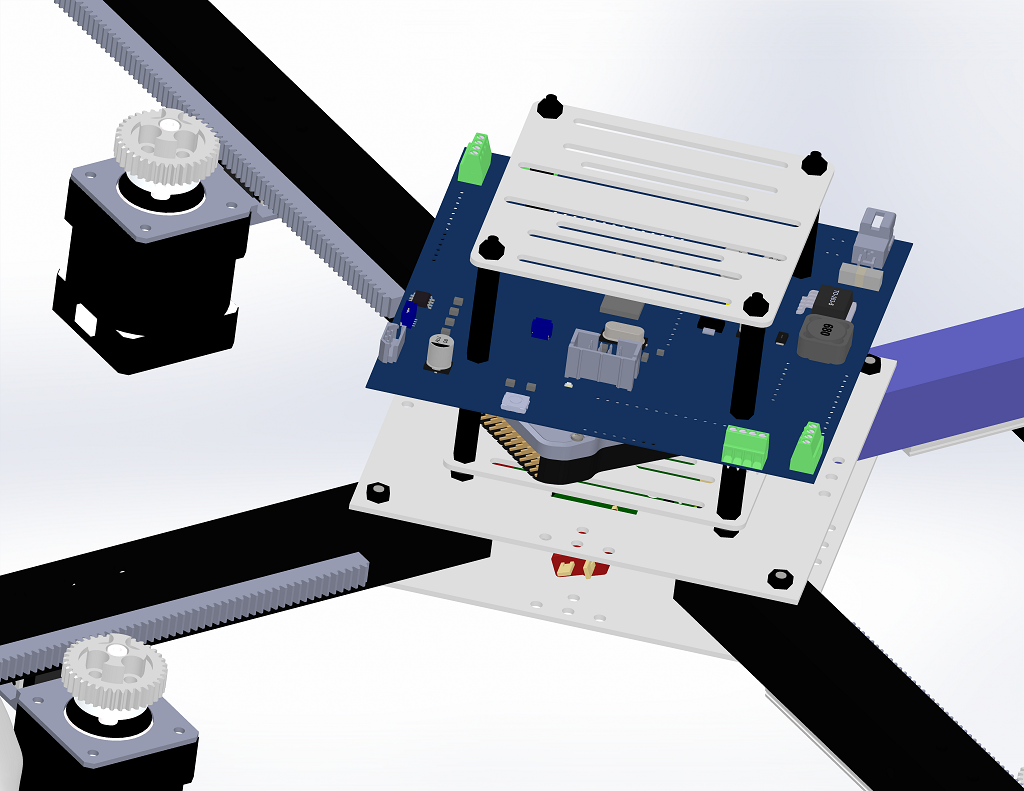
\includegraphics[width=0.7\textwidth]{figures/arducopter_slot_top.png}
	\caption{Sloj za proširenje}
	\label{fig:slot_top}
\end{figure}

\subsection{Prikaz rezalizacije mehaničke konstrukcije}
OVDJE STAVITI FOTOGRAFIJE STVARNE LETJELICE


\end{document}